\documentclass[11pt]{article}
\usepackage[utf8]{inputenc}
\usepackage[T1]{fontenc}
\usepackage{amsmath}
\usepackage{amssymb}
\usepackage{graphicx}
\usepackage{booktabs}
\usepackage{hyperref}
\usepackage{geometry}
\usepackage{xcolor}
\usepackage{caption}
\geometry{margin=1in}
\graphicspath{{figures/}}
\captionsetup{font=small}

\newcommand{\Qfull}{Q_{\mathrm{full}}}
\newcommand{\Qmix}{Q_{\mathrm{mix}}}

\title{%
  \textbf{SEARL with ConfGate Auxiliary Heads}\\[4pt]
  \large Results on CartPole, HalfCheetah and the Bike Environment}
\author{Technion NeuroAI Lab}
\date{\today}

\begin{document}
\maketitle

% ============================================================
\section{Summary}
% ============================================================
We replaced the RNN controller of the ConfGate experiments by SEARL (population-based evolution of a DQN),
and asked whether auxiliary heads that see only part of the observation help it, either by scaling the
learning rate (the ``lr gate'') or by also taking part in the choice of the action (``heads act'').
The heads never change the Q-network's own gradient. Main findings:

\begin{itemize}
  \item \textbf{HalfCheetah, SEARL + 2 heads (lr gate) vs.\ SEARL DQN.} The gated version ends higher in 9 of 10 paired
        seeds (mean difference $+900 \pm 414$, bootstrap 95\% CI $[+181, +1720]$). On CartPole there is no difference.
  \item \textbf{SEARL versus single-agent DQN.} SEARL learns fast but is unstable late in training. On CartPole it ends
        far below CleanRL DQN and Rainbow ($\approx 170$ vs.\ $\approx 450$--$490$ out of 500).
  \item \textbf{Heads that act do not give a reliable gain.} With 3 seeds, no arm is clearly better than the lr gate
        alone. For single-agent DQN, letting the heads act lowers the final level on both tasks.
  \item \textbf{Bike environment (252 runs).} No consistent winner. The heads change nothing for single-agent DQN;
        SEARL variants reach 95\% of the maximum earlier ($\approx 10$k steps vs.\ $\approx 20$k) but end lower and more
        variable on the harder boards. Rainbow has the highest final level in 9 of 12 settings.
  \item \textbf{Two failures were diagnosed.} The ``lr-only'' ablation never learns because the policy collapses to one
        action after the random phase (Section~\ref{sec:diag}). SEARL's late degradation is repeated collapses after a
        peak, not a smooth decay; it is not caused by the lr drift, and judging each individual on more episodes
        reduced it.
\end{itemize}
All comparisons use few seeds (3 unless stated), and the seed-to-seed spread is often as large as the gaps; claims
below are worded accordingly.

% ============================================================
\section{Methods}
% ============================================================

\subsection{SEARL DQN}
The base algorithm is a sequential reproduction of SEARL for a discrete-action DQN: a population of 4
networks (one hidden layer of 128 units, ReLU), a shared replay buffer, tournament selection of size 3 with elitism,
and the mutation operators of the original code. Each epoch every individual plays episodes with
$\epsilon = 0.1$ (fitness $=$ mean episode return, transitions go to the shared replay); after selection and mutation each
individual is trained with a double-DQN update (Huber loss, soft target update $\tau = 0.01$, Adam, batch 128,
initial lr $3\cdot10^{-4}$) for a number of steps proportional to the frames just collected. The first 5000 steps
use random actions. Each individual receives one of five operators with equal probability: no change, weight
perturbation, architecture growth, activation change, or an lr mutation (multiply by 1.2 or 0.8, clipped to
$[10^{-5}, 5\cdot10^{-3}]$).

\subsection{ConfGate auxiliary heads}
Each individual additionally carries $K$ linear heads on the Q-network's last hidden layer. Head $k$ is
fed an observation in which only its group of entries is kept and the rest is zeroed (mask $M_k$):
\[
  Q_k(s,\cdot) = W_k\,\phi(M_k s) + b_k ,
\]
where $\phi$ is the last hidden activation of the Q-network. The trunk is detached, so the heads do not change the
Q-network's gradient. After every TD phase the heads are fitted (Huber loss, own Adam) to the same TD target that
is computed from the full network, $y = r + \gamma(1-d)\max_{a'}\Qfull(s',a')$.

Two head layouts were used:
\begin{itemize}
  \item \textbf{2 heads} on observation groups: CartPole cart $=$ obs[0:2] and pole $=$ obs[2:4];
        HalfCheetah pose $=$ obs[0:8] and velocity $=$ obs[8:17]; bike left/right (Section~\ref{sec:bike}).
  \item \textbf{per-observation heads}: one head per observation entry (4 on CartPole, 17 on HalfCheetah).
\end{itemize}
HalfCheetah is discretised to 6 joints with 3 torques each (18 outputs, factored actions); every quantity below
is then computed per joint and averaged.

\paragraph{Confidence.} On a batch of $B$ replay states let $c_a(s)$ be the number of heads whose greedy action is $a$.
\[
  m = \frac{1}{B}\sum_{s}\ \sum_{a} \frac{c_a(s)\,(c_a(s)-1)}{K(K-1)} .
\]
For $K=2$ this is exactly the fraction of states on which the two heads pick the same action.

\paragraph{lr gate.} For one training phase the learning rate is
\[
  \mathrm{lr}_{\mathrm{eff}} = \mathrm{lr}_{\mathrm{base}}\,\bigl(f + \sigma\, m\bigr), \qquad f\in[0.2,1],\ \sigma\in[0,1],
\]
with initial $f=\sigma=0.5$. $\mathrm{lr}_{\mathrm{base}}$ is SEARL's own mutated learning rate and is restored after the
phase, so the gate never accumulates into the inherited value. The gate can only lower the learning rate. $f$ and $\sigma$
belong to the individual and are mutated by a sixth operator, \emph{controller} (Gaussian step proportional to the value,
$\mathrm{sd}=0.1$, clipped); every operator then has probability $1/6$. There is no controller gradient and no
feedback matrix. With $f=1,\sigma=0$ the run is bit-identical to plain SEARL (checked).

\paragraph{Heads act (mix).} In the ``heads act'' variants the action is chosen from
\[
  \Qmix(s,a) = (1-\lambda)\,\Qfull(s,a) + \lambda\,\frac{1}{K}\sum_{k} Q_k(s,a),\qquad \lambda\in[0,1],
\]
in the $\epsilon$-greedy fitness episodes and in the greedy evaluation. The TD target and the Q-network update are unchanged.
$\lambda$ is a per-individual coefficient, initialised to 0.2 and mutated by the controller operator with an
additive step $\lambda \leftarrow \mathrm{clip}(\lambda + \mathcal N(0, 0.1),0,1)$ (a multiplicative step could never
leave 0). It is inherited by clones; selection acts on fitness only. Two arms: \emph{mix only} (lr gate off) and
\emph{mix + lr gate} (the controller mutates $f$, $\sigma$ and $\lambda$ with equal probability). With $\lambda=0$ fixed
and the gate off the run is again bit-identical to plain SEARL (checked).

\subsection{Single-agent counterparts}
The same heads, confidence and gate were added to a CleanRL DQN with its own replay and $\epsilon$ schedule, without
population, mutation or selection. There is nothing to evolve, so $f=\sigma=0.5$ and (for the mix variants)
$\lambda = 0.2$ are fixed. With $f=1,\sigma=0$ the run is byte-identical to the original CleanRL baseline.

\subsection{Evaluation and seeds}
CartPole-v1 and discrete HalfCheetah-v4 were run for $10^6$ steps. SEARL variants use 10 seeds for
SEARL DQN and SEARL + 2 heads (lr gate), and 3 seeds for everything else; single-agent DQN and Rainbow use 10 seeds on
CartPole and 3 on HalfCheetah. The heads-act comparison uses 3 paired seeds for all arms (CartPole seeds 1--3,
HalfCheetah seeds 0--2).

\emph{Final level} is, per seed, the mean over the last 10\% of the budget of the greedy test return of SEARL's best
individual (one evaluation per epoch), or of the training-episode return for DQN and Rainbow; tables give mean $\pm$ sd
over seeds with the number of seeds in brackets. \textbf{The two metrics differ} (greedy evaluation versus training
episodes with exploration), so SEARL-versus-baseline gaps are not strictly like for like; comparisons within the SEARL
family and within the DQN family are.

% ============================================================
\section{CartPole and HalfCheetah: the lr gate}
% ============================================================
Table~\ref{tab:main} gives the final levels and Figure~\ref{fig:all} the learning curves.

\begin{table}[h]
\centering\small
\begin{tabular}{lrr}
\toprule
Variant & CartPole-v1 & HalfCheetah-v4 \\
\midrule
SEARL DQN & 167 $\pm$ 88 (10) & 794 $\pm$ 823 (10) \\
SEARL + 2 heads (lr gate) & 166 $\pm$ 59 (10) & 1694 $\pm$ 946 (10) \\
SEARL + per-obs heads (lr gate) & 194 $\pm$ 44 (3) & 1766 $\pm$ 447 (3) \\
\midrule
CleanRL DQN & 453 $\pm$ 35 (10) & 1673 $\pm$ 539 (3) \\
DQN + 2 heads (lr gate) & 465 $\pm$ 53 (10) & 1159 $\pm$ 334 (3) \\
DQN + per-obs heads (lr gate) & 475 $\pm$ 9 (3) & 1820 $\pm$ 264 (3) \\
\midrule
Rainbow & 487 $\pm$ 12 (10) & 1942 $\pm$ 347 (3) \\
\bottomrule
\end{tabular}
\caption{Final level, $10^6$ steps (mean $\pm$ sd over seeds, seeds in brackets).}
\label{tab:main}
\end{table}

\begin{table}[h]
\centering\small
\begin{tabular}{lrrrrr}
\toprule
Task & SEARL + 2 heads & SEARL DQN & mean diff $\pm$ s.e. & seeds ahead & bootstrap 95\% CI \\
\midrule
CartPole-v1 & 166 & 167 & -2 $\pm$ 33 & 5/10 & [-65, +58] \\
HalfCheetah-v4 & 1694 & 794 & +900 $\pm$ 414 & 9/10 & [+181, +1720] \\
\bottomrule
\end{tabular}
\caption{SEARL + 2 heads (lr gate) minus SEARL DQN, 10 paired seeds.}
\label{tab:paired}
\end{table}

\begin{itemize}
  \item On HalfCheetah the lr gate helps SEARL (Table~\ref{tab:paired}); the plain SEARL runs peak much higher than they
        end (per-seed peaks average $\approx 3100$ for SEARL DQN on the 3 paired seeds, against a final level of $\approx 880$)
        and the gate keeps more of it. On CartPole it makes no difference.
  \item SEARL rises faster than the DQN family early, then degrades late (Section~\ref{sec:diag}); on CartPole it ends
        far below CleanRL DQN and Rainbow. Rainbow has the highest final level on both tasks.
  \item In single-agent DQN, 2 heads with the gate end lower on HalfCheetah ($1159$ vs.\ $1673$) and similar on CartPole;
        per-observation heads end at or above the baseline on both, but with 3 seeds and sds of $260$--$540$ on HalfCheetah
        this is not a reliable gain.
  \item The gate does lower the learning rate (single-agent, 2 heads: about $0.75\times$ the base on CartPole and
        $0.71\times$ on HalfCheetah; per-observation heads about $0.91\times$ on HalfCheetah, where $m\approx 0.83$).
        In SEARL the base lr itself drifts down by about an order of magnitude on both tasks.
\end{itemize}

\begin{figure}[p]
\centering
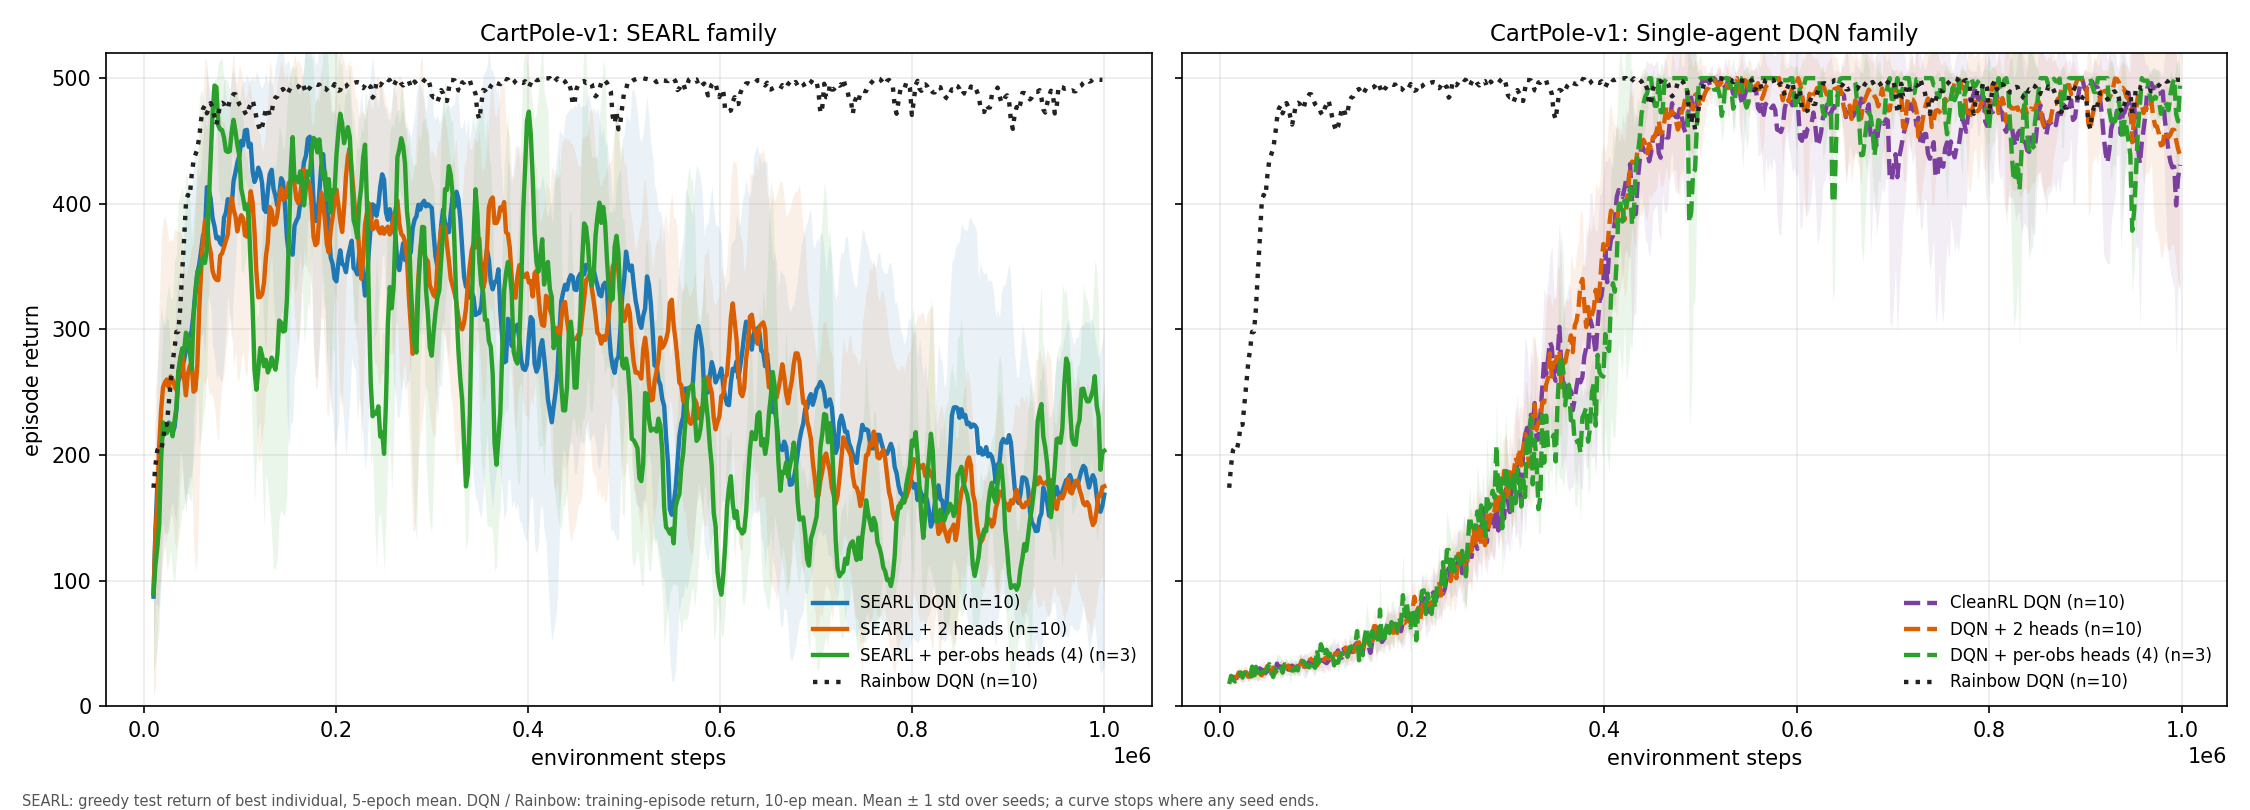
\includegraphics[width=\textwidth]{all_variants_cartpole_1M.png}\\[6pt]
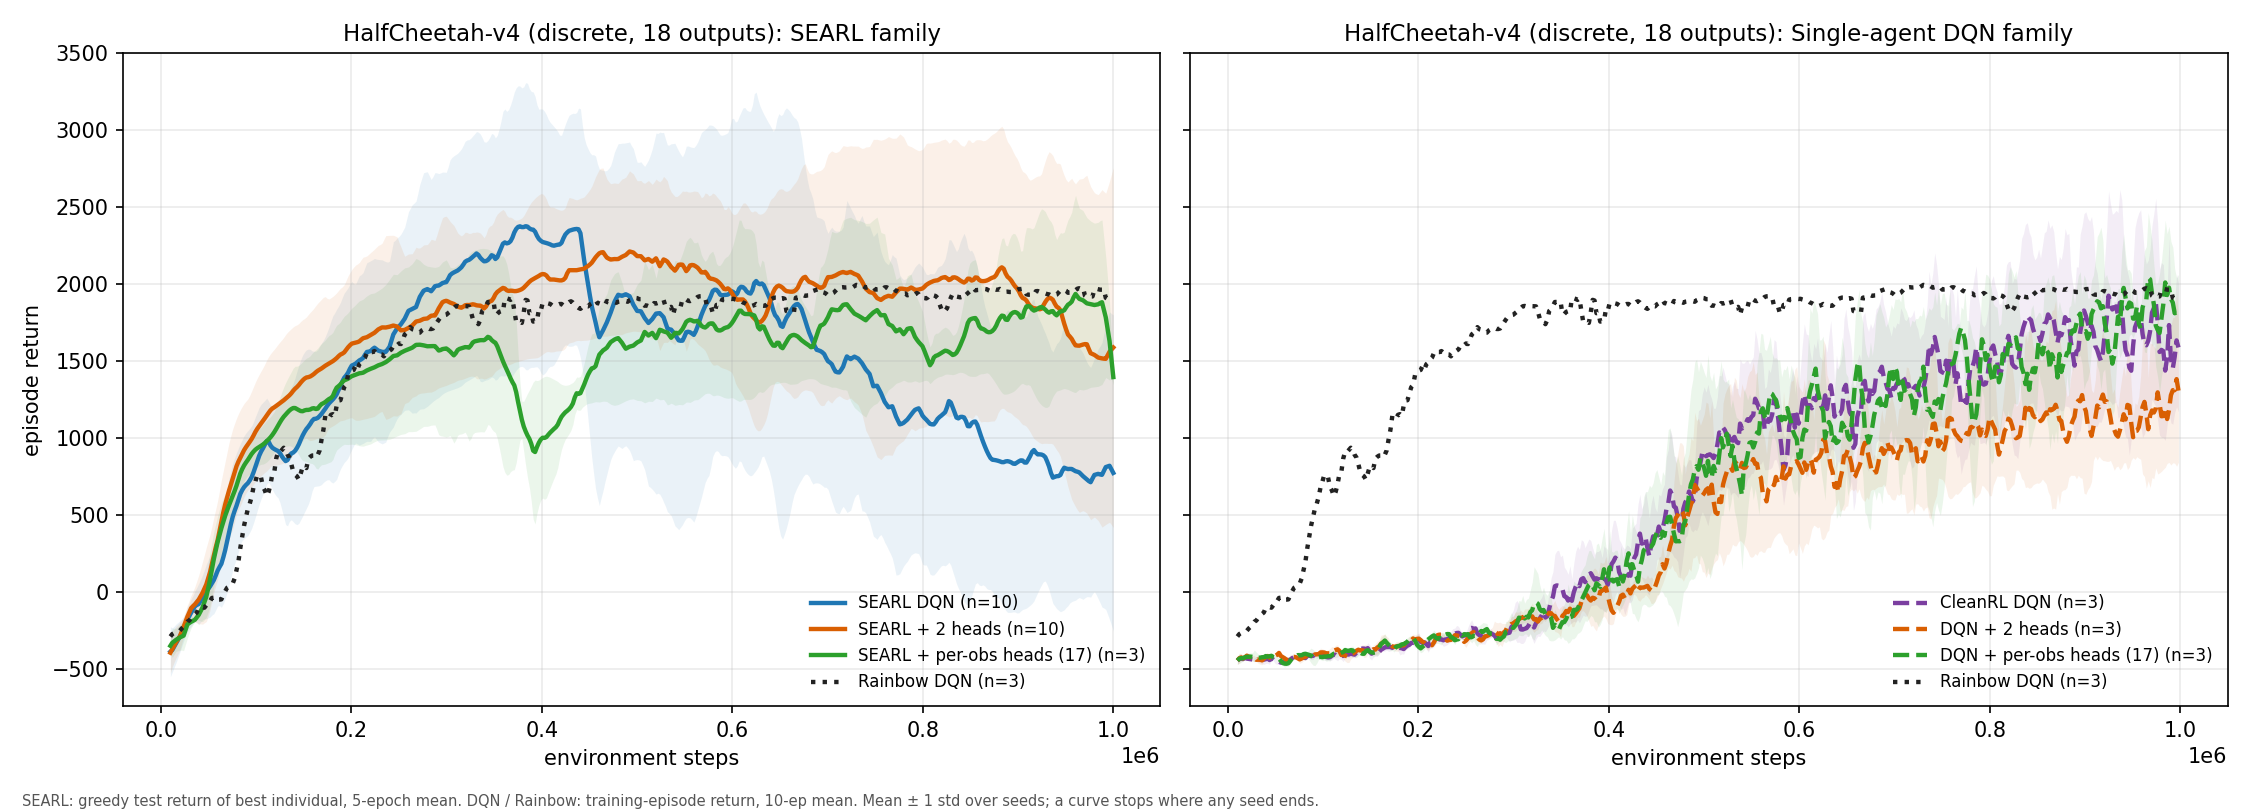
\includegraphics[width=\textwidth]{all_variants_halfcheetah_1M.png}
\caption{All variants, $10^6$ steps (mean $\pm$ 1 sd over seeds). Left: SEARL family; right: single-agent DQN family;
Rainbow for reference. SEARL curves are the greedy test return of the best individual, DQN and Rainbow curves are
training-episode returns.}
\label{fig:all}
\end{figure}

\begin{figure}[p]
\centering
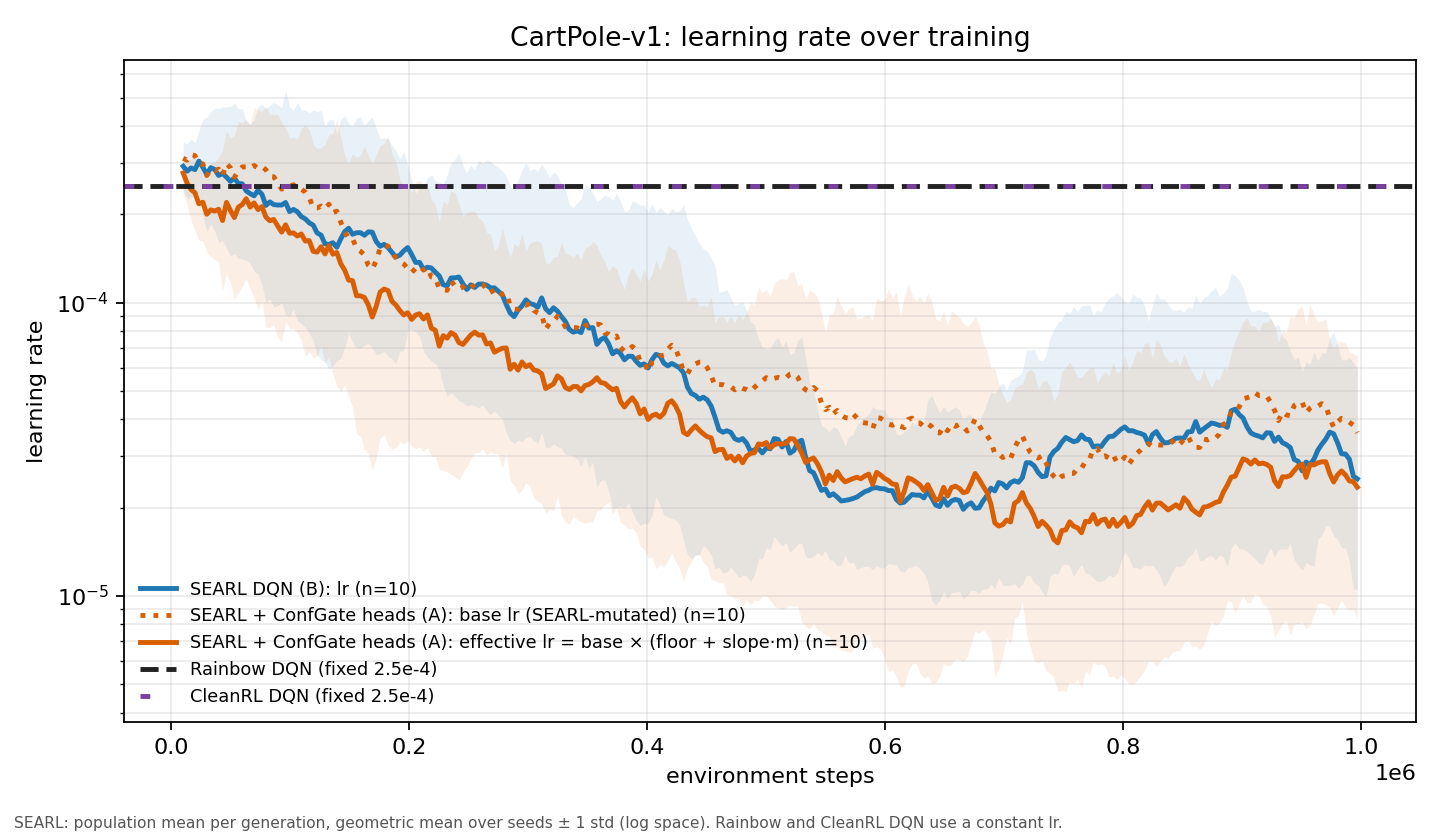
\includegraphics[width=0.78\textwidth]{lr_cartpole_1M.png}\\[6pt]
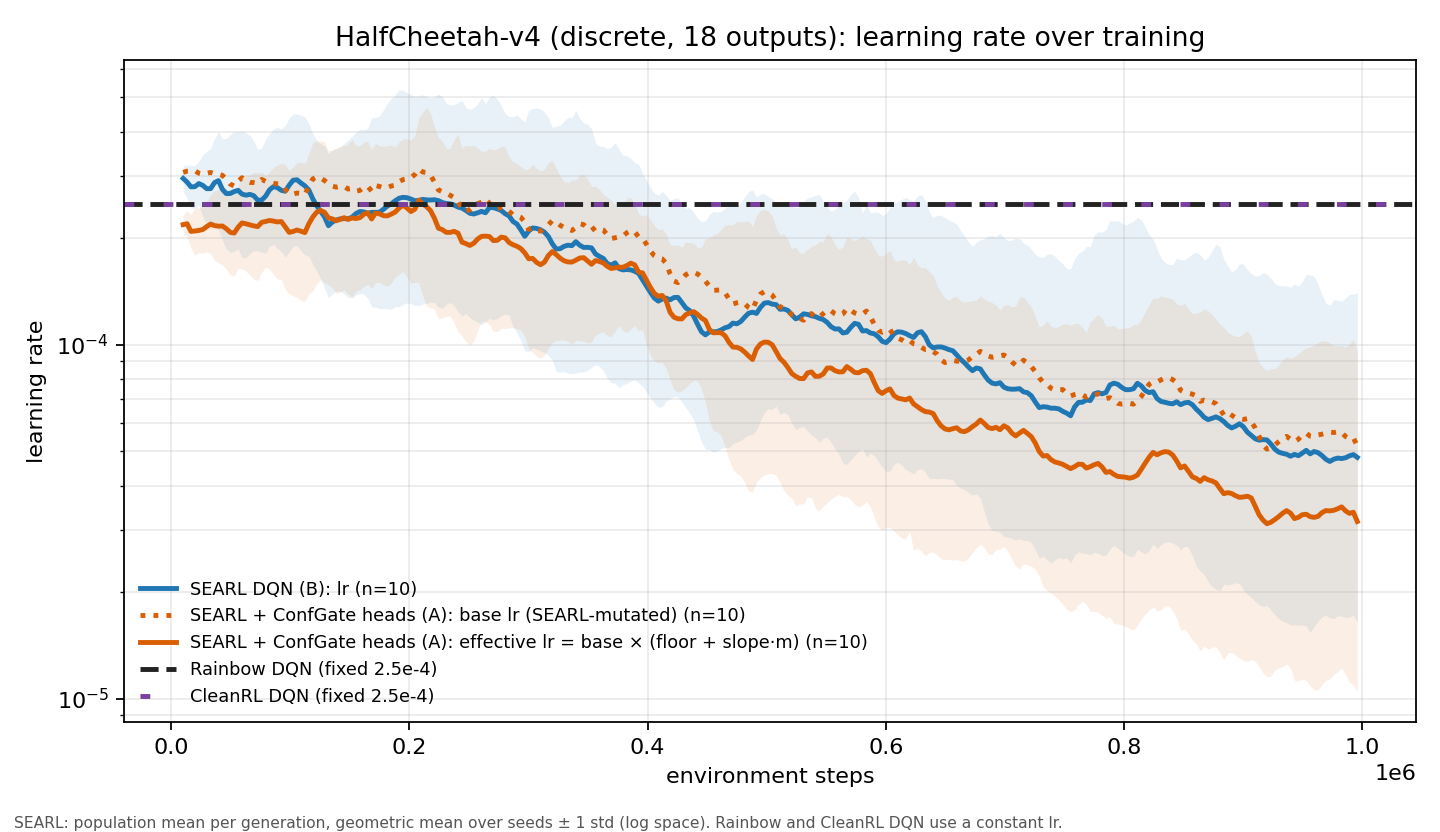
\includegraphics[width=0.78\textwidth]{lr_halfcheetah_1M.png}
\caption{Learning rate over training for the four algorithms (CartPole top, HalfCheetah bottom).}
\label{fig:lr}
\end{figure}

% ============================================================
\section{Heads that act}
% ============================================================
Table~\ref{tab:mix} compares the lr gate alone with the two heads-act arms, for SEARL and for the single-agent DQN, on 3
paired seeds. Figure~\ref{fig:mixcurves} shows the SEARL curves and Figure~\ref{fig:mixfinal} the per-seed final levels.

\begin{table}[h]
\centering\small
\begin{tabular}{llrr}
\toprule
Family & Variant & CartPole-v1 & HalfCheetah-v4 \\
\midrule
SEARL & no heads (SEARL DQN) & 169 $\pm$ 55 (3) & 882 $\pm$ 939 (3) \\
SEARL & 2 heads, lr gate only & 169 $\pm$ 75 (3) & 1718 $\pm$ 746 (3) \\
SEARL & 2 heads, heads act (mix only) & 167 $\pm$ 138 (3) & 586 $\pm$ 1110 (3) \\
SEARL & 2 heads, heads act + lr gate & 194 $\pm$ 48 (3) & 1743 $\pm$ 1484 (3) \\
SEARL & per-obs heads, lr gate only & 194 $\pm$ 44 (3) & 1766 $\pm$ 447 (3) \\
SEARL & per-obs heads, heads act (mix only) & 276 $\pm$ 79 (3) & 1393 $\pm$ 1045 (3) \\
SEARL & per-obs heads, heads act + lr gate & 109 $\pm$ 11 (3) & 425 $\pm$ 1102 (3) \\
\midrule
single-agent DQN & no heads (CleanRL DQN) & 454 $\pm$ 17 (3) & 1673 $\pm$ 539 (3) \\
single-agent DQN & 2 heads, lr gate only & 435 $\pm$ 86 (3) & 1159 $\pm$ 334 (3) \\
single-agent DQN & 2 heads, heads act (mix only) & 305 $\pm$ 50 (3) & 847 $\pm$ 121 (3) \\
single-agent DQN & 2 heads, heads act + lr gate & 316 $\pm$ 61 (3) & 952 $\pm$ 232 (3) \\
single-agent DQN & per-obs heads, lr gate only & 475 $\pm$ 9 (3) & 1820 $\pm$ 264 (3) \\
single-agent DQN & per-obs heads, heads act (mix only) & 297 $\pm$ 122 (3) & 647 $\pm$ 187 (3) \\
single-agent DQN & per-obs heads, heads act + lr gate & 397 $\pm$ 101 (3) & 544 $\pm$ 285 (3) \\
\bottomrule
\end{tabular}
\caption{Heads-act variants, final level at $10^6$ steps, 3 paired seeds.}
\label{tab:mix}
\end{table}

\begin{itemize}
  \item \textbf{No arm is reliably better.} In SEARL the curves overlap and cross, and the seed spread ($\pm 50$ to $\pm 1500$)
        is as large as any gap.
  \item \textbf{CartPole.} SEARL with per-observation heads, mix only, ends highest in the SEARL family ($276$ vs.\ $169$
        for SEARL DQN; all three seeds are above the SEARL DQN mean), but the same heads with the lr gate added are the
        lowest ($109$). The two uses of the heads do not add up.
  \item \textbf{HalfCheetah.} The heads-act arms do not beat the lr gate alone. Several seeds end negative, and in most arms one or two seeds fail while another does well, so single seeds decide the mean.
  \item \textbf{Single-agent DQN.} With $\lambda=0.2$ fixed, letting the heads act lowers the final level on both tasks
        (CartPole $297$--$397$ vs.\ $454$; HalfCheetah $544$--$952$ vs.\ $1673$). A plausible reason is that the heads see
        only part of the observation, but this was not tested.
\end{itemize}

\begin{figure}[p]
\centering
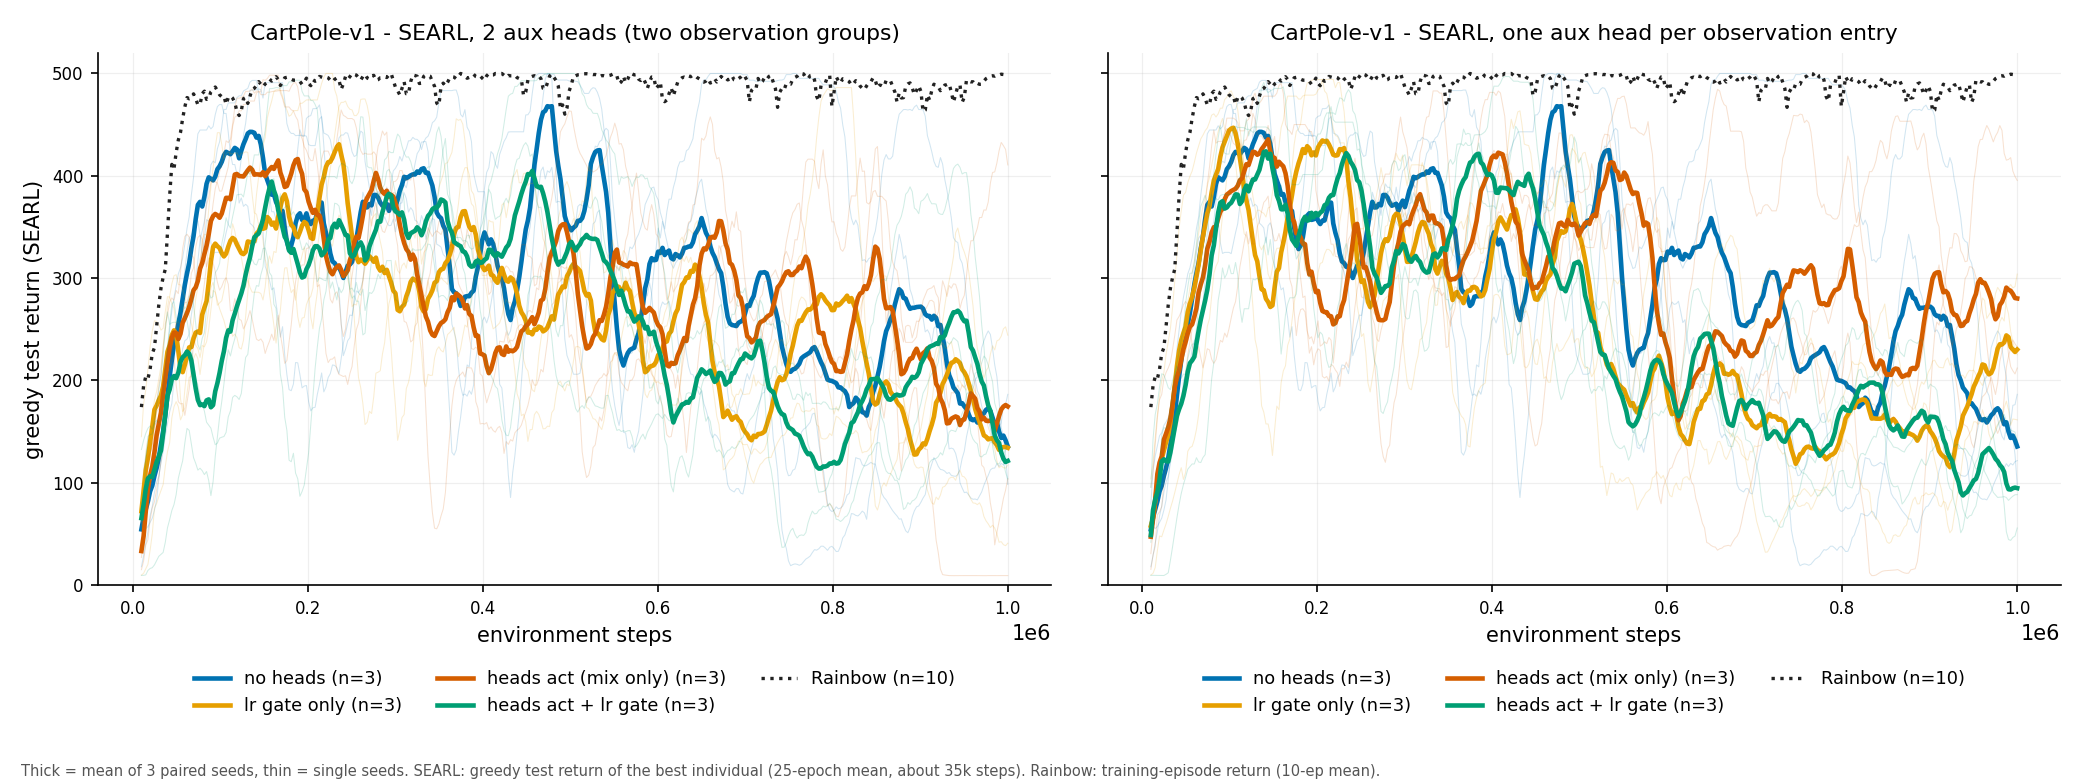
\includegraphics[width=\textwidth]{mix_curves_cartpole.png}\\[6pt]
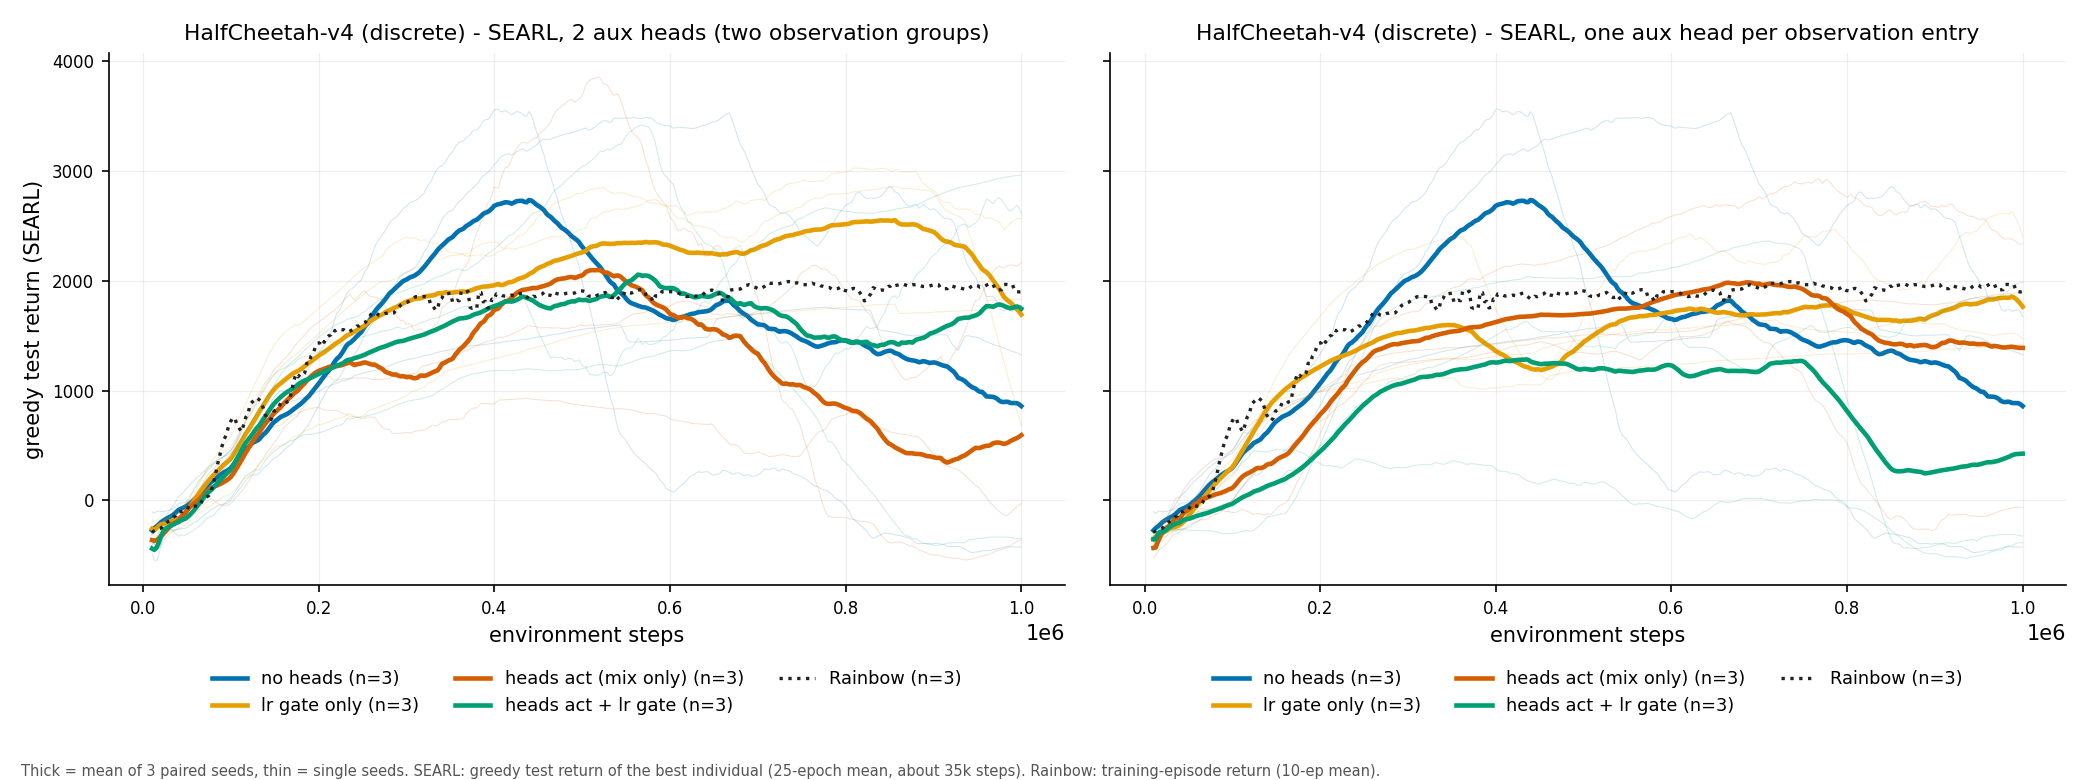
\includegraphics[width=\textwidth]{mix_curves_halfcheetah.png}
\caption{SEARL, heads-act variants, 3 paired seeds (thick: mean, thin: seeds). Left: 2 heads; right: per-observation heads.
SEARL curves are smoothed over 25 epochs ($\approx$ 35k steps); Rainbow is shown for reference.}
\label{fig:mixcurves}
\end{figure}

\begin{figure}[p]
\centering
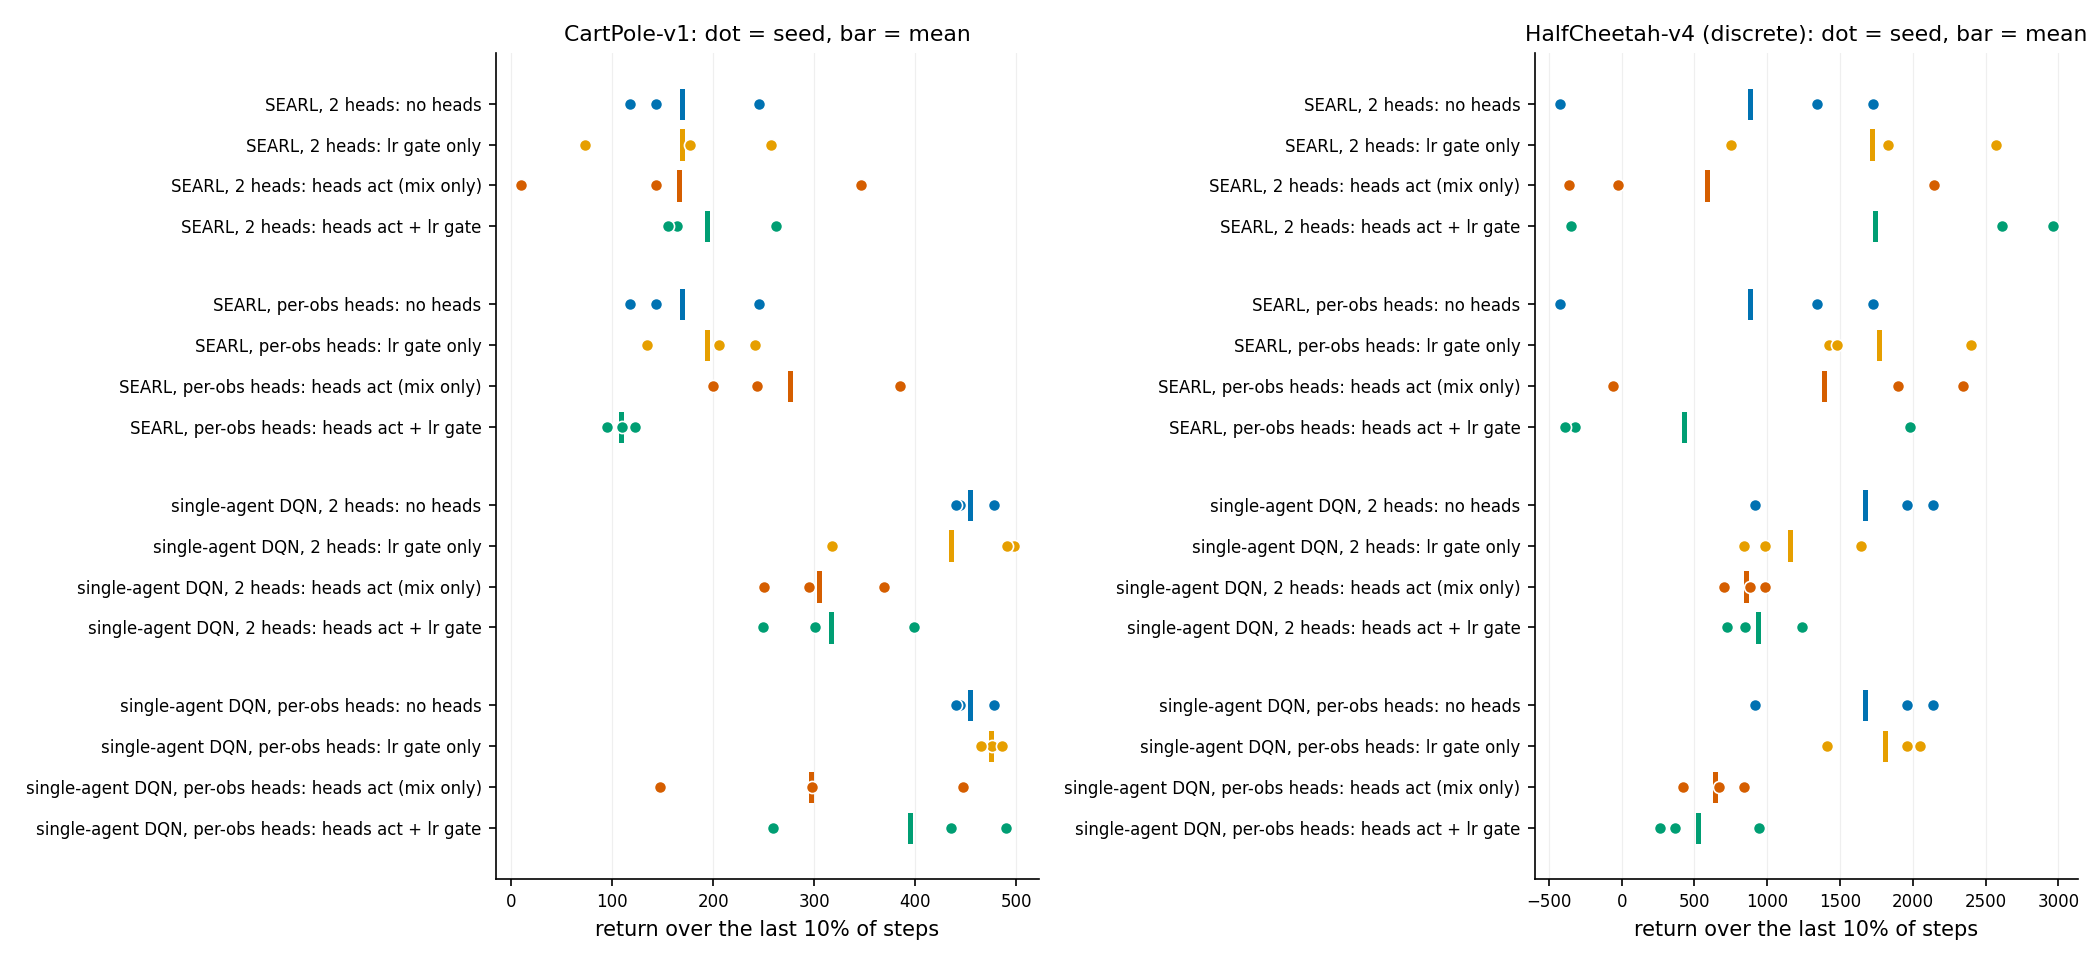
\includegraphics[width=\textwidth]{mix_final_levels.png}
\caption{Final level per seed (dot) and mean (bar) for every variant, SEARL and single-agent.}
\label{fig:mixfinal}
\end{figure}

\subsection{What SEARL does with $\lambda$}
Figure~\ref{fig:lambda} and Table~\ref{tab:lambda} show $\lambda$, averaged over the 4 individuals.
The direction depends on the task and on whether the lr gate is on. On CartPole $\lambda$ rises in 3 of the 4 arms
(the exception is 2 heads with the lr gate); on HalfCheetah it falls or stays low in 3 of the 4
(per-observation heads with the gate stay near 0.2 on average, but their seeds end at 0, 0.56 and 0.14).
\textbf{This is not evidence that selection raises $\lambda$ when the heads help.} With 3 seeds, a rise or fall may be
the random walk of the mutation; a control in which $\lambda$ mutates but selection ignores it was not run.

\begin{table}[h]
\centering\footnotesize
\begin{tabular}{llrrl}
\toprule
Task & Variant & $\lambda$ first 10\% & $\lambda$ last 10\% & final $\lambda$ per seed \\
\midrule
CartPole-v1 & 2 heads, heads act (mix only) & 0.10 & 0.51 & 0.65, 0.12, 0.75 \\
CartPole-v1 & 2 heads, heads act + lr gate & 0.24 & 0.12 & 0.02, 0.00, 0.33 \\
CartPole-v1 & per-obs, heads act (mix only) & 0.13 & 0.47 & 0.23, 0.71, 0.48 \\
CartPole-v1 & per-obs, heads act + lr gate & 0.11 & 0.41 & 0.51, 0.47, 0.25 \\
HalfCheetah-v4 & 2 heads, heads act (mix only) & 0.17 & 0.19 & 0.05, 0.45, 0.08 \\
HalfCheetah-v4 & 2 heads, heads act + lr gate & 0.22 & 0.01 & 0.01, 0.01, 0.02 \\
HalfCheetah-v4 & per-obs, heads act (mix only) & 0.23 & 0.07 & 0.13, 0.09, 0.00 \\
HalfCheetah-v4 & per-obs, heads act + lr gate & 0.21 & 0.23 & 0.00, 0.56, 0.14 \\
\bottomrule
\end{tabular}
\caption{$\lambda$ in the first and last 10\% of training phases (mean over 3 seeds and the 4 individuals) and per seed at the end.}
\label{tab:lambda}
\end{table}

\begin{figure}[h]
\centering
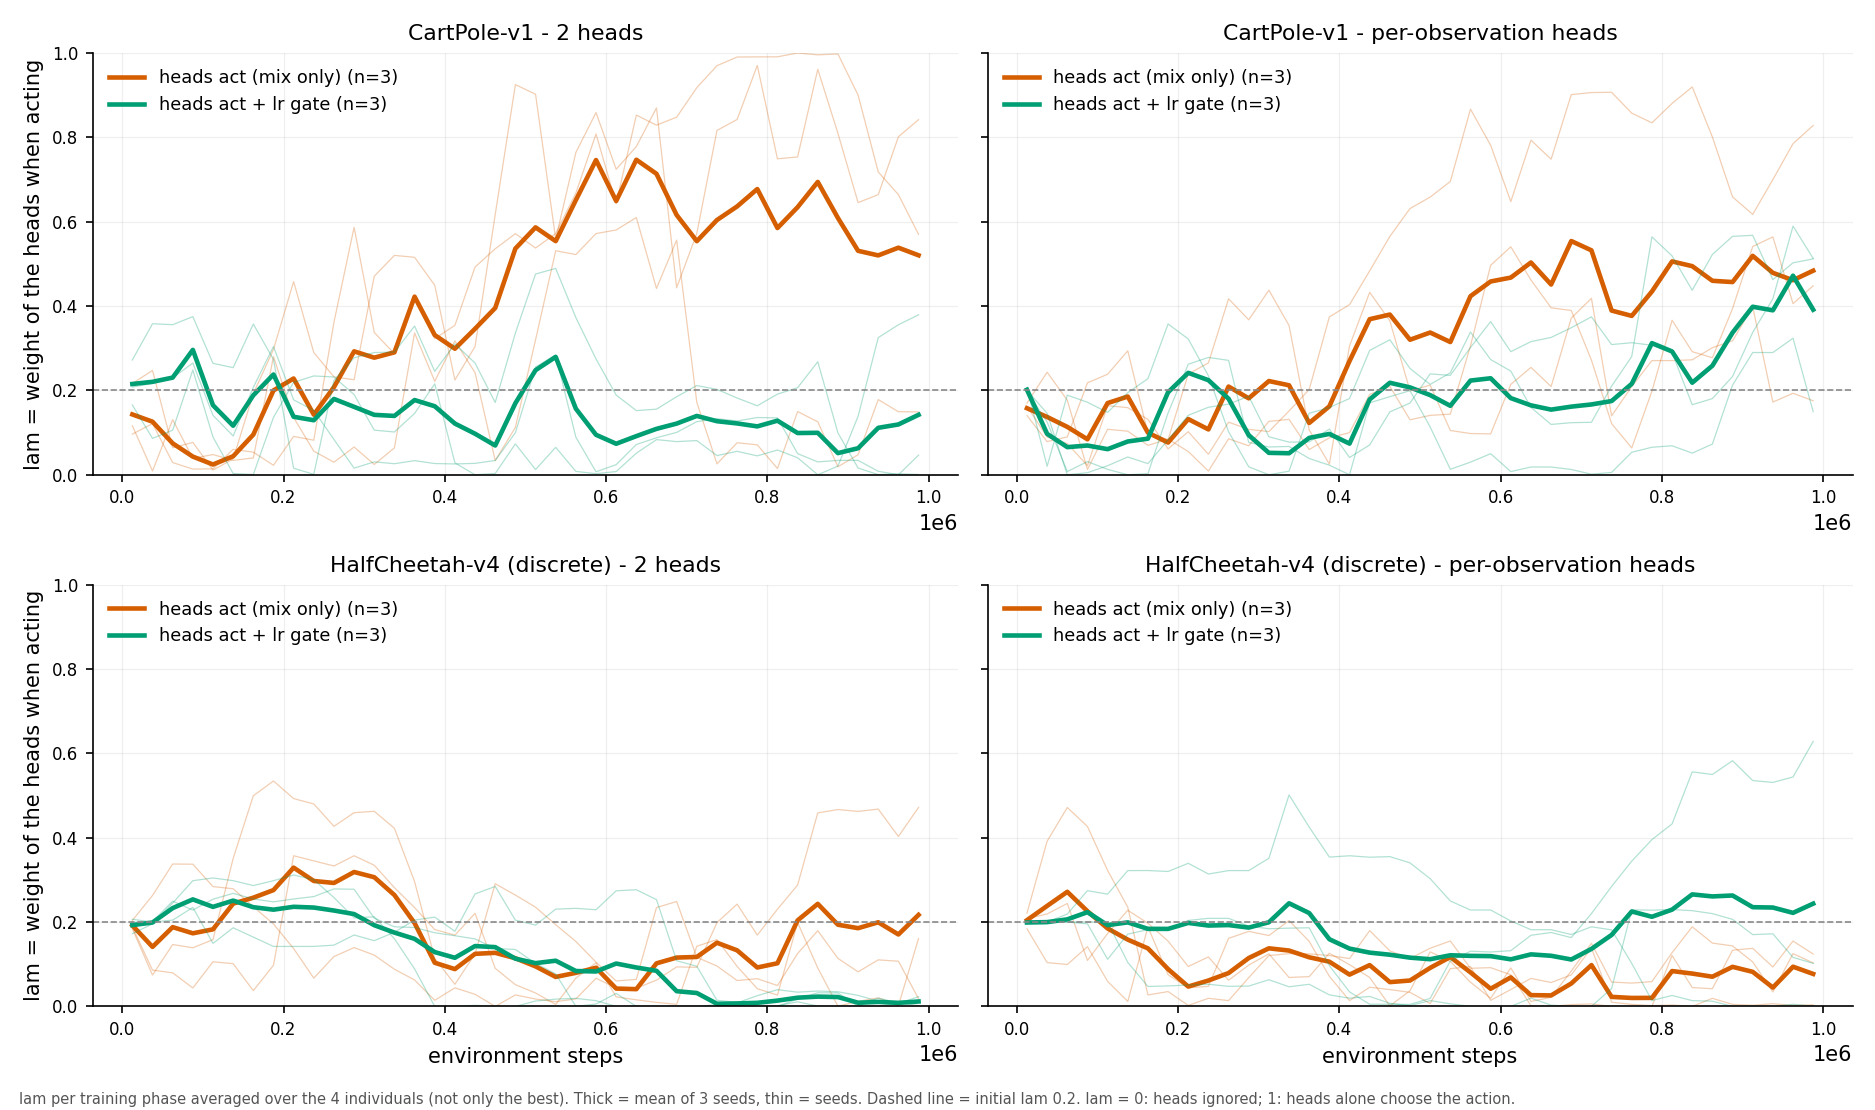
\includegraphics[width=0.92\textwidth]{mix_lambda.png}
\caption{$\lambda$ over training (thick: mean of 3 seeds, thin: seeds). Dashed: initial value 0.2.}
\label{fig:lambda}
\end{figure}

% ============================================================
\section{Bike environment}\label{sec:bike}
% ============================================================
All seven variants (SEARL DQN, SEARL + 2 heads, SEARL + per-observation heads, CleanRL DQN, DQN + 2 heads,
DQN + per-observation heads, Rainbow) were run on the bike environment (v2.1) with 2, 3, 5 and 10 lanes and 1, 8 and 100
solutions (the number of fall-free routes; fewer solutions is harder), 3 seeds, 480k steps: 252 runs. The observation is
the speed, the distance to the nearest hole in each lane, and ego-relative lane slots (4, 5, 8, 16 numbers for 2, 3, 5, 10 lanes),
with 3 actions. The two heads see the speed, the bike's own slot, and the slots to the left, respectively to the right; the
per-observation version has one head per entry.

To compare all variants as fairly as possible, every method is evaluated by the same procedure: a greedy
(no exploration) evaluation on 10 fixed fresh boards (reset seeds 5000--5009) about every 10k steps, in its own
environment (not counted as training steps and not stored). The final level is the mean of the last 5 evaluations.
Earlier, an SB3 DQN had reached the maximum return (4900) on every lanes $\times$ solutions combination.

\begin{table}[h]
\centering\small
\begin{tabular}{rrrrrrrrr}
\toprule
Lanes & Sol. & S & S+2h & S+obs & DQN & D+2h & D+obs & Rb \\
\midrule
2 & 1 & 4886 & 4813 & 4895 & 4853 & 4883 & 4887 & \textbf{4900} \\
2 & 8 & 4789 & \textbf{4894} & \textbf{4894} & 4842 & 4877 & 4879 & 4719 \\
2 & 100 & 4875 & \textbf{4897} & 4879 & 4887 & 4882 & 4874 & 4855 \\
\addlinespace
3 & 1 & 4824 & 4868 & 4371 & 4872 & \textbf{4887} & 4886 & 4885 \\
3 & 8 & 4814 & 4855 & 4860 & 4876 & 4885 & 4879 & \textbf{4885} \\
3 & 100 & 4860 & 4874 & 4855 & 4838 & 4874 & 4888 & \textbf{4891} \\
\addlinespace
5 & 1 & 4871 & 4848 & 4812 & 4867 & 4882 & 4852 & \textbf{4900} \\
5 & 8 & 4775 & 4256 & 4253 & 4818 & 4878 & 4871 & \textbf{4894} \\
5 & 100 & 4769 & 4783 & 4234 & 4865 & 4860 & 4879 & \textbf{4894} \\
\addlinespace
10 & 1 & 4711 & 4846 & 4745 & 4862 & 4742 & 4835 & \textbf{4880} \\
10 & 8 & 4559 & 4472 & 4661 & 4841 & 4818 & 4811 & \textbf{4900} \\
10 & 100 & 4517 & 4740 & 4143 & 4851 & 4836 & 4758 & \textbf{4893} \\
\bottomrule
\end{tabular}
\caption{Bike environment, final greedy return (maximum 4900), mean over 3 seeds, best of each row in bold.
S $=$ SEARL DQN, S+2h / S+obs $=$ SEARL with 2 / per-observation heads (lr gate), DQN $=$ CleanRL DQN,
D+2h / D+obs the single-agent counterparts, Rb $=$ Rainbow.}
\label{tab:bike}
\end{table}

\begin{itemize}
  \item \textbf{The heads change nothing for single-agent DQN.} The three DQN variants are within about 120 of each other in
        every setting (and within 50 in most).
  \item \textbf{SEARL is faster but less stable.} All three SEARL variants reach 95\% of the maximum in about 10k steps at 2--5 lanes
        (about 20k for the DQN variants), but on harder boards they end lower and more variable (e.g.\ 5 lanes with 8 solutions: 4256 and 4253 for SEARL with 2 and with per-observation heads;
        5 lanes with 100 solutions: 4234 and 10 lanes with 100 solutions: 4143, both for per-observation heads).
  \item \textbf{Heads versus no heads inside SEARL flips by setting}, so no consistent effect can be claimed.
  \item \textbf{Rainbow has the highest final level in 9 of 12 settings}, with the largest dip at 2 lanes with 8 solutions (4719).
\end{itemize}

\begin{figure}[p]
\centering
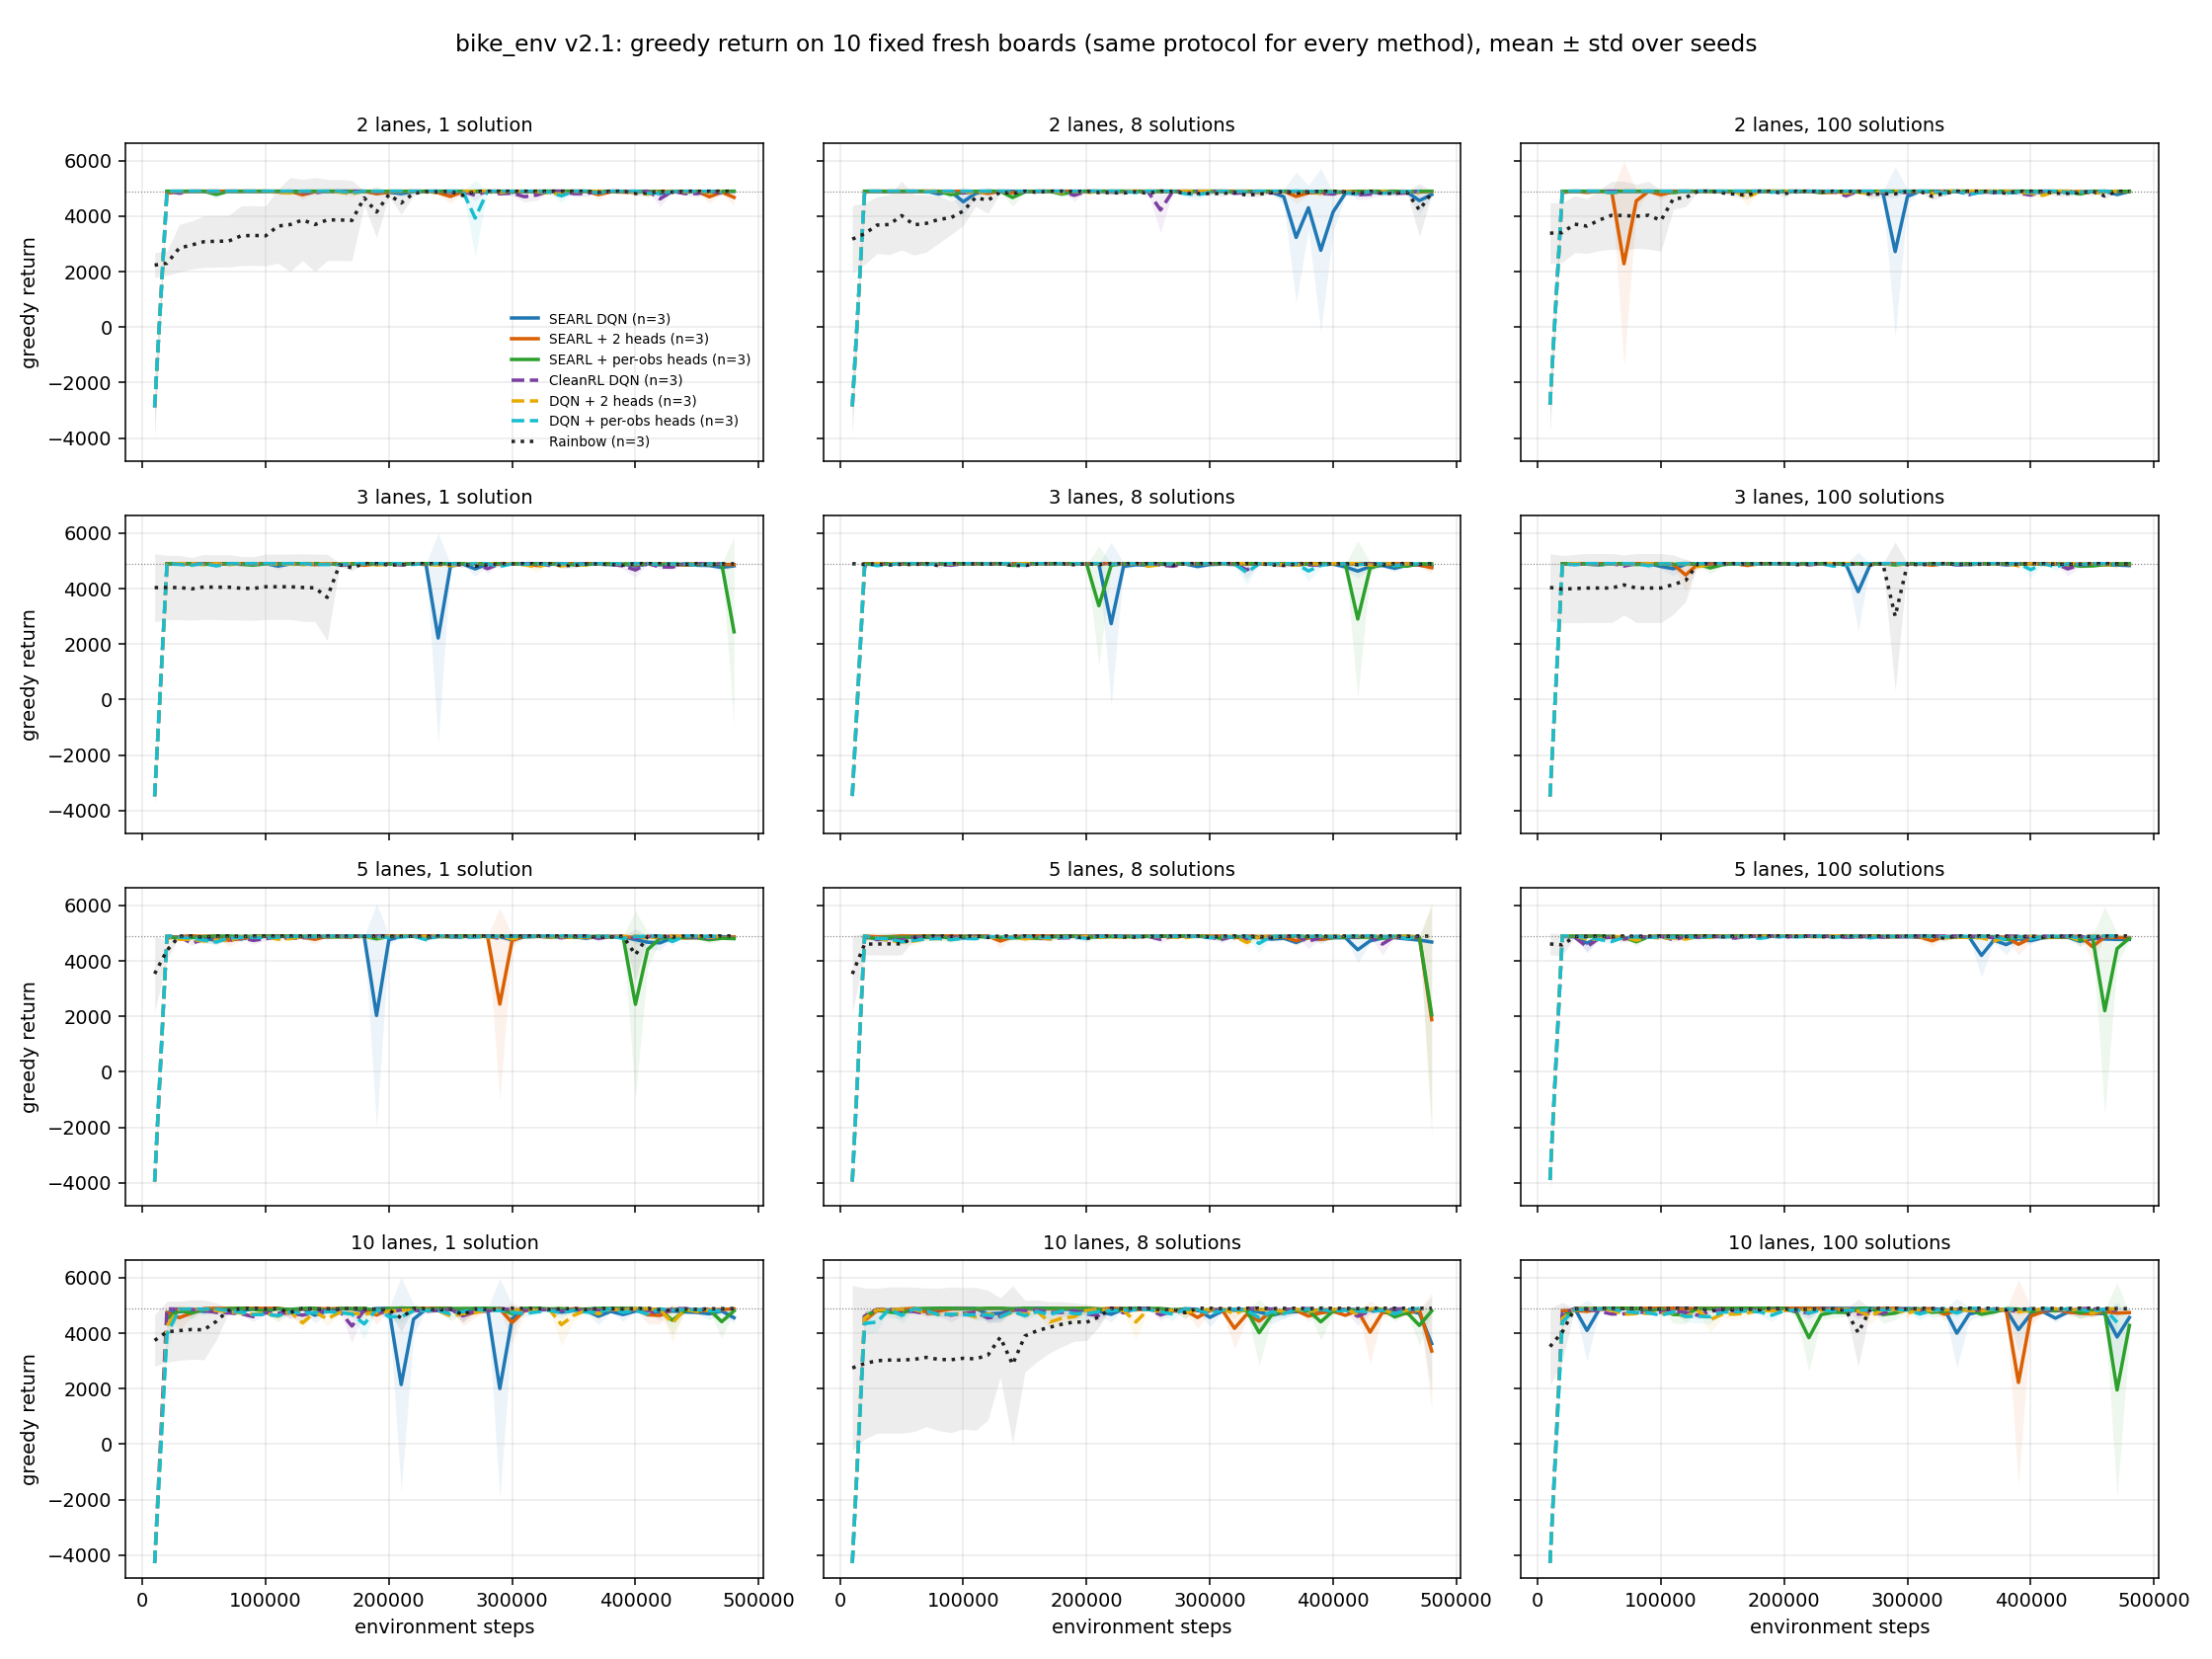
\includegraphics[width=\textwidth]{bike_grid_curves.png}
\caption{Bike environment, greedy return over training for all variants, one panel per lanes $\times$ solutions setting.}
\label{fig:bikegrid}
\end{figure}

% ============================================================
\section{Why SEARL fails: two diagnoses}\label{sec:diag}
% ============================================================
Both diagnoses use controlled CartPole runs of plain SEARL (no controller), 4 seeds per variant, with the same code as above.

\subsection{The lr-only ablation never learns}
In the lr-only ablation the weight, architecture and activation mutations are switched off. All 20 runs of the earlier
500k-step ablation ended at a return of about 9. In the first epoch after the 5000-step random phase the first trained
network becomes a constant-action policy; the replay then holds 90--95\% of a single action in episodes of about 10 steps,
so nothing teaches the Q-network the other action, and the fixed $\epsilon = 0.1$ is too little to repair it. Table~\ref{tab:lronly}
shows that more exploration does not help and that adding the weight mutation helps only partly. Full SEARL escapes the trap;
we believe the architecture and activation mutations do it, but these were not tested separately.

\begin{table}[h]
\centering\small
\begin{tabular}{lcc}
\toprule
Variant (100k frames, seeds 1--4) & best test return per seed & mean of last 20 evaluations \\
\midrule
lr only, $\epsilon=0.1$            & 10, 10, 10, 22 & 9, 9, 9, 9 \\
lr only, $\epsilon=0.3$            & 10, 10, 10, 22 & 9, 9, 9, 9 \\
lr + weight mutation               & 62, 40, 10, 72 & 9, 9, 9, 20 \\
\bottomrule
\end{tabular}
\caption{The lr-only collapse. Fraction of replay actions equal to one action after the random phase: 0.95 / 0.05 (per seed)
at $\epsilon=0.1$ and 0.85 / 0.15 at $\epsilon=0.3$.}
\label{tab:lronly}
\end{table}

\subsection{Late degradation}
SEARL does not decay smoothly: it reaches 400--500 at about 100--200k steps and afterwards collapses repeatedly
(for example $450 \to 61 \to 443 \to 12$ on one seed) while its base lr drifts down to about $10^{-5}$.
Table~\ref{tab:degr} compares five variants over 500k steps. A ``collapsed evaluation'' is a greedy test return below 100
after the run's 10-evaluation mean first exceeded 300.

\begin{table}[h]
\centering\small
\begin{tabular}{lccc}
\toprule
Variant & mean last 100k (per seed) & mean & collapsed evals (mean) \\
\midrule
plain SEARL                       & 135, 323, 337, 278 & 268 & 26 \\
no lr mutation (lr fixed)         & 217, 305, 363, 211 & 274 & 36 \\
no weight mutation                & 335, 373, 364, 255 & 332 & 21 \\
5$\times$ fewer updates per frame & 199, 325, 310, 264 & 274 & 15 \\
5 evaluation episodes per individual & 450, 473, 273, 271 & 367 & 9 \\
\bottomrule
\end{tabular}
\caption{Late degradation, CartPole, 500k steps, 4 seeds per variant.}
\label{tab:degr}
\end{table}

\begin{itemize}
  \item \textbf{The lr drift is not the cause:} with the lr fixed at $3\cdot10^{-4}$ the collapses persist (and are no rarer).
  \item The lower update ratio gives fewer collapses but no better last-100k mean; we read this as a weak or no effect.
  \item \textbf{Noisy selection is the best-supported explanation, but is not proven.} Judging each individual on about 5 instead of
        about 1 episodes gave the best last-100k mean ($367$ vs.\ $268$) and the fewest collapses ($9$ vs.\ $26$); one of its
        four seeds still collapsed badly.
  \item Not tested: the replay holding the whole history uniformly, and a mutated elite.
\end{itemize}
With 4 seeds and a seed-to-seed sd of about 100, differences between variants of less than about 100 are not significant.

% ============================================================
\section{Limitations}
% ============================================================
\begin{itemize}
  \item Few seeds (3 for most comparisons); most gaps are within the seed spread. The one comparison with 10 seeds shows an
        effect only on HalfCheetah.
  \item SEARL curves are greedy test returns of the best individual, while the DQN and Rainbow curves are training-episode returns.
  \item Whether the changes in $\lambda$ reflect selection or random drift is not established (no blind-selection control).
  \item The heads-act variants were run on CartPole and HalfCheetah only; the bike runs use the lr gate but not heads that act.
  \item The explanation of SEARL's late degradation is partial (Section~\ref{sec:diag}).
\end{itemize}

\end{document}
